% !TEX root = ../../../main.tex

\toggletrue{image}
\toggletrue{imagehover}
\chapterimage{genetic_algorithms}
\chapterimagetitle{\uppercase{Genetic Algorithms}}
\chapterimageurl{https://xkcd.com/534/}
\chapterimagehover{Just make sure you don't have it maximize instead of minimize.}

\chapter{Funktionen}
\label{ch:funktionen}

Mit eigenen Funktionen machen wir unsere Programme übersichtlicher und verständlicher. Wir können damit auch auf Tastatur- und Mausereignisse reagieren. Die Lernziele sind:\\

\lernziel{\autoref{ch:funktionen}, \nameref{ch:funktionen}}{
\begin{minipage}{\linewidth}
$\square$ \hspace{0.1cm} Sie erklären, was eine Funktion ist und warum die Verwendung nützlich sein kann.\\
$\square$ \hspace{0.1cm} Sie geben Beispiele für bestehende Funktionen.\\
$\square$ \hspace{0.1cm} Sie definieren eine Funktion in Python und rufen diese an geeigneter Stelle auf.\\
$\square$ \hspace{0.1cm} Sie verwenden Funktionen, um Code bei einem Tastaturereignis auszuführen.
\end{minipage}
}

\vspace{-0.5cm}

\section{Zwei Quadrate \Winkey}

Wir können mit dem Programm aus \autoref{lst-zwei-quadrate-funktion} die Figur aus \autoref{figure-zwei-quadrate-funktion} zeichnen.

\begin{figure}[htb]
\centering
\begin{minipage}[c][4cm]{0.5\linewidth}
\centering
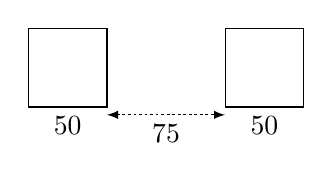
\begin{tikzpicture}
	\draw (0,0) to node [sloped,below] {$50$} ++(1cm, 0) -- ++(0, 1cm) -- ++(-1cm, 0) -- ++(0, -1cm);
	\draw (2.5cm,0) to node [sloped,below] {$50$} ++(1cm, 0) -- ++(0, 1cm) -- ++(-1cm, 0) -- ++(0, -1cm);
	\draw[latex-latex, thin, dashed, dash pattern=on 1pt off 1pt] (1cm,-0.1cm) to node [sloped, below] {$75$} ++(1.5cm, 0);
\end{tikzpicture}
\caption{Zwei Quadrate mit Abstand $75$.}
\label{figure-zwei-quadrate-funktion}
\end{minipage}
\hfill
\begin{minipage}[c]{0.4\linewidth}
\centering
\begin{lstlisting}[language={python3}, caption={\graybgtexttt{zwei\_quadrate.py}}, label={lst-zwei-quadrate-funktion}]
import turtle as t


def quadrat_<@\color{black}{50}@>():
	for _ in range(4):
		t.fd(50)
		t.lt(90)


quadrat_<@\color{black}{50}@>()
t.pu()
t.fd(125)
t.pd()
quadrat_<@\color{black}{50}@>()

t.done()

\end{lstlisting}
\end{minipage}
\end{figure}

\vspace{-0.5cm}

Wir gestalten den Code übersichtlich und sparen Tipparbeit, indem wir eine Funktion definieren und zweimal aufrufen.

\vfill

\begin{definition}[Funktion]
Mit einer Funktion fassen wir Quellcode unter einem \textbf{Namen} zusammen und verwenden ihn an mehreren Stellen wieder, ohne den Code kopieren zu müssen.
\end{definition}

\newpage

\autoref{lst-zwei-quadrate-funktion} zeigt die Verwendung einer Funktion am Beispiel der beiden Quadrate. Bisher haben wir \say{nur} bestehende Funktionen aufgerufen. Nun definieren wir zunächst eigene Funktionen und rufen diese dann auf. \autoref{figure-funktionen-aufbau} zeigt diesen Zusammenhang.

\begin{figure}[htb]
\centering
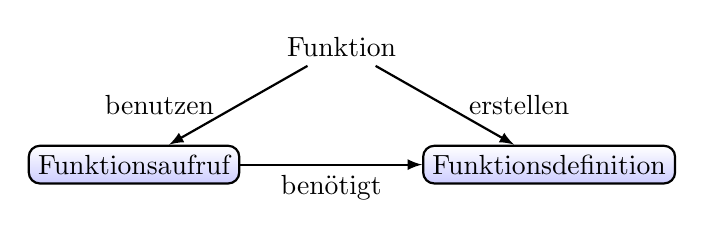
\begin{tikzpicture}[sibling distance=15em, edge from parent/.style = {draw, -latex, thick}]
  \node {Funktion}
    child {	 node[{shape=rectangle, thick, rounded corners,
    draw, align=center, top color=white, bottom color=blue!20}] (call) {Funktionsaufruf} edge from parent node [left, xshift=-0.5em] {benutzen}}
    child { node[{shape=rectangle, thick, rounded corners,
    draw, align=center, top color=white, bottom color=blue!20}] (def) {Funktionsdefinition} edge from parent node [right, xshift=0.5em] {erstellen}};
  \path[-latex, draw, thick] (call) edge node[below] {benötigt} (def);
\end{tikzpicture}
\caption{Aufbau von Funktionen}
\label{figure-funktionen-aufbau}
\end{figure}

\begin{important}[Funktionsdefinition $\neq$ Funktionsaufruf]
Grundsätzlich gilt: Bevor eine Funktion aufgerufen werden kann, muss sie definiert werden. Wenn man eine Funktion definiert, dann werden die Befehle der Funktion noch \textbf{nicht} automatisch ausgeführt.
\end{important}

\section{Funktionsdefinition}

Eine Funktionsdefinition besteht aus einem \textbf{Funktionskopf} und einem \textbf{Funktionskörper}. Zuerst wird der Funktionskopf notiert, dann der Funktionskörper. \autoref{lst:funktionsdefinition-struktur} zeigt den allgemeinen Aufbau einer Funktionsdefinition und \autoref{lst:funktionsdefinition-beispiel} ein konkretes Beispiel einer Funktionsdefinition.

\begin{figure}[H]
\centering
\begin{minipage}{0.4\textwidth}
\begin{lstlisting}[language={python3}, caption={Allgemeine Struktur}, label={lst:funktionsdefinition-struktur}]


def FUNKTIONSNAME():
	BEFEHL <@\color{black}{1}@>
	BEFEHL <@\color{black}{2}@>
	...


\end{lstlisting}
\end{minipage}
\hfill
\begin{minipage}{0.55\textwidth}
\centering
\begin{lstlisting}[language={python3}, caption={Beispiel einer Funktionsdefinition}, label={lst:funktionsdefinition-beispiel}]


def quadrat_<@\color{black}{50}@>():
	for _ in range(4):
		t.fd(50)
		t.lt(90)


\end{lstlisting}
\end{minipage}
\end{figure}

\vspace{-0.75cm}

\subsection{Funktionskopf}

Der Funktionskopf beginnt \textbf{immer} mit dem Schlüsselwort\footnote{Wir haben bereits weitere Schlüsselwörter kennengelernt: \lstinline[language={python3}]{import}, \lstinline[language={python3}]{for} und \lstinline[language={python3}]{in}.} \lstinline[language={python3}]{def} (eine Abkürzung für \textbf{definition}). Das Schlüsselwort \lstinline[language={python3}]{def} bedeutet, dass nun die Definition der Funktion beginnt. Der Funktionskopf \textbf{muss} mit einem Doppelpunkt \lstinline[language={python3}]{:} abgeschlossen werden.

\subsection{Funktionskörper}

Nur die \textbf{eingerückten} Befehle gehören zum Funktionskörper und damit zur Funktionsdefinition. Diese Befehle werden beim Aufruf der Funktion ausgeführt. Innerhalb des Funktionskörpers können beliebige Befehle notiert werden.

\cleancoderegel{\autoref{ch:funktionen}, \nameref{ch:funktionen}}{
\begin{cleancode}[Leerzeilen bei der Funktionsdefinition]
Vor \textbf{und} nach einer Funktionsdefinition sind \textbf{zwei Leerzeilen} einzufügen.
\end{cleancode}
}

\vspace{-0.65cm}

\cleancoderegel{\autoref{ch:funktionen}, \nameref{ch:funktionen}}{
\begin{cleancode}[Einrückung 2]
Die Einrückung (engl. indentation) des \textbf{Funktionskörpers} erfolgt mit der Tabulatortaste.
\end{cleancode}
}

\section{Funktionsaufruf}

Mit einem \textbf{Funktionsaufruf} können wir eine \textbf{Funktion ausführen}. Ein Funktionsaufruf erfolgt durch die Notation des \textbf{Funktionsnamens} und der \textbf{Klammern}. Den Funktionsaufruf kennen wir schon. Wir haben schon immer Funktionen aufgerufen, die \textit{andere} Programmierer geschrieben haben. Neu ist nun, dass wir auch noch unsere eigenen Funktionen aufrufen.

\begin{example}
Ausgewählte Funktionsaufrufe bereits vorhandener Funktionsdefinitionen:
\begin{multicols}{2}
\begin{itemize}
\item \lstinline[language={python3}]{forward(100)}
\item \lstinline[language={python3}]{left(90)}
\item \lstinline[language={python3}]{pencolor("red")}
\item \lstinline[language={python3}]{randrange(50, 101)}
\item \lstinline[language={python3}]{choice(["red", "green", "blue"])}
\item \lstinline[language={python3}]{sqrt(42)}
\end{itemize}
\end{multicols}
\end{example}

\vspace{-0.5cm}

\begin{hinweis}
Der Funktionsaufruf eigener Funktionen unterscheidet sich nicht vom bisherigen Funktionsaufruf. Wir verwenden \textbf{weder} \lstinline[language={python3}]{def} beim Funktionsaufruf noch den Doppelpunkt. Einziger Unterschied: Unsere Funktionsdefinitionen haben noch keine Parameter für den Funktionsaufruf mit einem Argument. Aber auch das können wir noch hinzufügen.
\end{hinweis}

\vspace{-0.25cm}

Wir können eine Funktion beliebig oft aufrufen. Egal wann wir eine Funktion aufrufen, die Befehle innerhalb des Funktionskörpers werden immer genau einmal pro Funktionsaufruf ausgeführt.

\begin{important}
Wenn sich die Funktionsdefinition in derselben Python-Datei wie der Funktionsaufruf befindet, ist keine  \lstinline[language={python3}]{import}-Anweisung erforderlich. Die Funktion kann direkt aufgerufen werden. Andernfalls ist die übliche Notation mit dem \say{Punkt} zu verwenden.
\end{important}

\begin{example}[Zwei Quadrate]

In \autoref{lst-zwei-quadrate-funktion} rufen wir zweimal unsere eigene Funktion auf. In Zeile \num{10} und \num{14}: \lstinline[language={python3}, mathescape]!quadrat_$\color{black}{\texttt{50}}$!.

\end{example}

\vspace{-0.85cm}

\section{Funktionen kombinieren}

Natürlich können wir auch mehrere Funktionen definieren und die Funktionsaufrufe miteinander kombinieren. \autoref{lst-vier-quadrate-funktion} zeigt eine Erweiterung des Beispiels aus \autoref{lst-zwei-quadrate-funktion}.

\begin{lstlisting}[language={python3}, caption={Zwei Funktionsdefinitionen. In der zweiten Funktionsdefinition wird die erste Funktion durch die Schleife mehrfach aufgerufen.}, label={lst-vier-quadrate-funktion}]
import turtle as t


def quadrat_<@\color{black}{50}@>():
	for _ in range(4):
		t.fd(50)
		t.lt(90)


def quadrate():
	for _ in range(4):
		quadrat_<@\color{black}{50}@>()
		t.pu()
		t.fd(175)
		t.lt(90)
		t.pd()


quadrate()
t.done()

\end{lstlisting}

\section{Wie wählen wir Funktionsnamen?}

Im Rahmen der üblichen Regeln sind wir bei der Wahl des Funktionsnamens grundsätzlich frei. Allerdings sollten wir den Funktionsnamen so wählen, dass allein aus dem Funktionsnamen ersichtlich ist, was die Befehle im Funktionskörper bewirken.

\cleancoderegel{\autoref{ch:funktionen}, \nameref{ch:funktionen}}{
\begin{cleancode}[Sinnvolle Funktionsnamen]
Wir wählen \textbf{Funktionsnamen} so, dass wir sofot verstehen, was die Funktion macht. Wir verwenden keine Grossbuchstaben und trennen einzelne Wörter durch einen Unterstrich (\lstinline[language={python3}]{_}). Dadurch machen wir den Code \textbf{lesbarer}.
\end{cleancode}
}

\begin{example}[Zwei Quadrate]

Der Funktionsname \lstinline[language={python3}, mathescape]!quadrat_$\color{black}{\texttt{50}}$! aus \autoref{lst-zwei-quadrate-funktion} deutet direkt darauf hin, was die Funktion macht: Es wird ein Quadrat mit der Seitenlänge $50$ gezeichnet.

\end{example}

\vspace{-0.5cm}

\section{Tastaturereignisse verarbeiten}

Mit der Funktion \lstinline[language={python3}]{onkeypress} registrieren wir eine \textbf{Funktion}, die beim Drücken der entsprechenden Taste einmalig ausgeführt wird. Wird die Taste zweimal hintereinander gedrückt, wird die Funktion zweimal hintereinander ausgeführt. Das \textbf{erste Argument} ist der \textbf{Funktionsname}, das \textbf{zweite Argument} ist die \textbf{Tastenbezeichnung} als \textbf{String}. Damit die Tastaturereignisse verarbeitet werden, müssen wir \textbf{nach der Registrierung einmal} die \lstinline[language={python3}]{listen}-Funktion aufrufen.

\begin{lstlisting}[language={python3}, caption={\protect\lstset{language=python3} Es werden drei Funktionen registriert. Wenn wir zum Beispiel auf die Taste \protect\say{f} drücken, dann wird die Funktion \lstinline{move_forward_randomly} ausgeführt.}, label={lst-quadrate-funktion-tastatur}]
import turtle as t
import random as r


def quadrat_<@\color{black}{50}@>():
	for _ in range(4):
		t.fd(50)
		t.lt(90)


def move_forward_randomly():
	t.pu()
	laenge = r.randrange(100, 201)
	t.fd(laenge)
	t.pd()


def rotate_left_randomly():
	t.pu()
	winkel = r.randrange(0, 361)
	t.lt(winkel)
	t.pd()


t.onkeypress(quadrat_<@\color{black}{50}@>, "q")
t.onkeypress(move_forward_randomly, "f")
t.onkeypress(rotate_left_randomly, "l")
t.listen()
t.done()

\end{lstlisting}